\setlength{\headheight}{15pt}
\addtolength{\topmargin}{-2.5pt}

\chapter{Technology Review}

This section will provide an overview of the technologies chosen for the project. It was chosen based on the project requirements. 
The technologies used in the project are as follows:

\section{Executive Dashboard}
When it came to developing the Executive Dashboard for data analysis it was crucial to select the tools that could transform data into easily comprehensible information. After conducting research and exploring alternatives Angular and Chart.js were chosen for specific reasons.

\subsection{Angular}
Angular is based on TypeScript and often used for building single-page applications (SPAs) or enterprise-level solutions. It is a powerful tool for building
client-side web applications.

\subsubsection{Main Concepts: Components, Modules and Services}
Angular is composed of three foundational blocks: Components, Modules and services.

\subsubsection{Components} Components are like Lego blocks of the application. Each component holds a portion of the user interface and its behaviour. Components serve as the bridge between the application data and what the user experiences on the screen.\cite{angular-components}

\subsubsection{Modules} In Angular modules serve as containers that group related components, directives, and services together that can be combined with other modules. It plays an important role in improving maintainability and re-usability, key concepts of Angular development.\cite{angular-modules}

\subsubsection{Services} Angular services use typescript classes with injectable decorators. The decorator informs Angular that the class function as a service
and can be injected into other components that need that service.\cite{angular-services}
\subsection{Angular architecture} 
The Model-View-Controller (MVC) has as its components the model, the view, and the controller. With controller orchestrating the communication and
interactions between the model and the view.

\begin{figure}[ht]
    \centering
    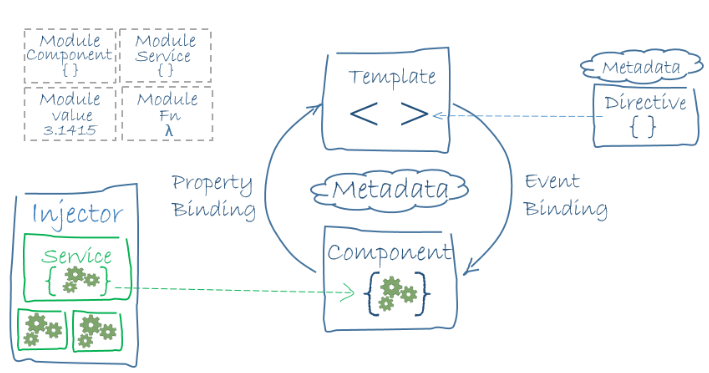
\includegraphics[width=0.85\linewidth]{images/angular-arch.png}
    \caption{Angular application architecture}
    \label{fig:angular-arch}
\end{figure}

\subsection{Advantages of using Angular}
\subsubsection{Component-Based Architecture}
As mentioned earlier in discussions Angular organizes its functionalities into components. These components have the ability to communicate with each other enabling updates to sections without affecting the rest of the application.

\subsubsection{Mobile-Friendly Approach}
Angular incorporates techniques such, as lazy-loading, which means loading parts of the application (like images) only when they are needed. This ensures that users do not experience long waiting times.

\subsubsection{Two-Way Data Binding}
Data can be synchronized between the model and the view. The two-way data binding feature in Angular ensures that any changes made to the model are reflected 
in the view and vice versa. 

\subsubsection{Asynchronous Programming}
By utilizing programming executes code in a non-sequential manner and employs multi-threading to enhance performance. This speeds up operations and prevents system freezes, providing users with a seamless experience.

\subsubsection{Single-Page Applications}
Angular creates a dynamic single-page application which can be navigated without page reloads, improving the user experience with better user interaction and engagement.

\subsubsection {Code Re-usability}
The component-based architecture of Angular promotes the re-usability of UI components saving development time.

\subsubsection{Dependency Injection}
With dependency injection in place, Angular allows for the creation of objects that rely on other objects. This improves modularity and efficiency, within the app.

\subsubsection{Angular Material}
Angular's documentation offers a range of built user interface components and modules that adhere to Google's Material Design principles. This greatly facilitates the developer's work, simplifying the design process and enabling application development.

\subsubsection{Angular CLI} Angular command line interface gives the developer the ability to generate Angular projects, modules, services, and components with a single command, 

which helps reduce configuration errors and gives the developer the freedom to dive into creative aspects of the project, focusing on innovation and functionality rather than getting bogged down by initial setup complexities.


\section{Data Visualization}

The visual representation of data is a important aspect of the project. It is used to communicate information clearly and efficiently. 
It allows to identify patterns, and find correlations that would be hard to identify in raw data, standing as an essential step in the data analysis process.

\subsection{Chart.js}


Chart.js is an efficient JavaScript library, it is not only open-source but also offers capabilities where attractive charts and graphs can be generated, and later
embedded into web pages. Chart.js became very popular due to its simplicity and ease of use, making it an excellent choice for data visualization tasks. Utilizing HTML5 
canvas technology, it ensures that charts are responsive and adjust seamlessly to the container's dimensions. Additionally, it boasts compatibility across 
all contemporary web browsers and enjoys support from an extensive developer community. Chart.js acts as an artist's palette for developers, equipped with 
a versatile API that supports an array of chart types, including line, radar, and pie charts, among others. Moreover, it provides extensive customization 
possibilities, enabling the creation of distinct and eye-catching charts.\cite{da2019learn}

Table \ref{tab:chart-js-features} is showing some of the features of Chart.js\cite{da2019learn}:

\begin{table}[H]
    \centering

    \begin{tabularx}{\textwidth}{|l|X|}
        \hline
        \textbf{Feature}            & \textbf{Description}                                                                                                                                                                                                \\
        \hline
        Easy to use                 & Aesthetically charts can be created without the need of extensive configuration. The library follows a declarative approach allowing the developer to define the data and settings of the chart in a single object. \\
        \hline
        Responsive                  & Charts generated by Chart.js are responsive, adapting to different devices, and makes sure that the visualization is readable across various platforms.                              \\
        \hline
        Customization               & Chart.js provides a high degree of customization. Colors, fonts, and other visual elements can be changed creating unique charts.                                                      \\
        \hline
        Interactivity               & Chart.js has great support tooltips and animation, enabling the user to explore the data points, adding a layer of engagement to the project.                                                               \\
        \hline
        Cross-browser compatibility & Chart.js is compatible with all most of the browsers.                                                                                                 \\
        \hline
    \end{tabularx}
    \label{tab:chart-js-features}
    \caption{Chart.js Features}
\end{table}

Chart.js stands as a dependable and powerful solution for visualizing data, with simple and intuitive APIs that facilitate the creation of attractive and
informative charts. Tt also benefits from the strong support of an extensive developer community, offering a significant advantage.


\section{AI module - Data analysis}

An amazing fact is that ninety percent of the data generated in the world was generated in the last two years. In the early 2000s, the amount of data being
generated exploded exponentially on the same rates as the internet and social media usage. Organizations found themselves facing a massive volume of data 
that was very hard to process. Then the concept of Big data was created to describe this large volume of data. It refers to data that is so large and complex
that traditional methods of data processing are not sufficient to process it. \cite{bigdata}


\subsection{Scikit-learn}

Scikit-learn, also know as sklearn, is an open-source machine-learning library for Python. It offers a range of regression and classification algorithms,
such as SVM, Random Forest, Gradient Boosting, and K-means. Its architecture allows it to be integrated with other Python libraries, such as NumPy, providing 
comprehensive toolkit for machine learning. \cite{scikit}

\begin{itemize}
    \item \textbf{Simple and Efficient Tools}: Scikit-learn offers a simple solution for data mining and data analysis.
    \item \textbf{Consistent Interface}: It provides an interface for the user that is consistent across different algorithms, so it is easy to switch between the models.
    \item \textbf{Integration}: Scikit-learn provides a wide range of algorithms and tools for machine learning which integrates seamlessly with other Python libraries.
    \item \textbf{Extensive Documentation}: With a large available community, the library has a huge documentation available, making it easy to find help and resources.
\end{itemize}

Scikit-learn was used on the AI model to train and evaluate machine learning models. As our dataset was in a structured format, Scikit-learn was the ideal choice for the project, 
providing algorithms that can be used to work with structured data. It was a regression problem, and for that, Linear Regression, Support Vector Machine,
Random Forest, and K-Nearest Neighbors algorithm from this library were used to evaluate the best model for the dataset.

\subsection{TensorFlow}

TensorFlow was developed by the Google Brain team and has been widely adopted in the machine learning community. It mainly used for deep learning tasks, such as neural networks, and machine
learning that requires a large amount of data. It is not only powerful but also flexible, allowing for the creation of custom machine learning models. It is also highly scalable, allowing for 
the training of models on multiple CPUs, GPUs, and TPUs (Tensor Processing Units).\cite{tensorflow}

\begin{itemize}
    \item \textbf{Flexible Architecture}: 
    \item TensorFlow provides developers with the capability to execute computations across multiple CPUs or GPUs using a unified API, whether on desktops, servers, or mobile devices, thereby making it versatile for various applications.
    \item \textbf{Comprehensive Library}: 
    \item This platform offers libraries and community support, that enables the developer to create and implement applications powered by ML.
    \item \textbf{High-Level APIs}: With high-level APIs like Keras, TensorFlow is very accessible to any developer, simplifying the build of the models. It also provides a low-level API for more advanced users, allowing for greater flexibility and customization.
    \item \textbf{Visualization with TensorBoard}: As part of TensorFlow, there is a tool called TensorBoard, which provides many visualization tools that are great to aid the understanding
    of the model, debugging, and optimization of complex neural networks.
    \item \textbf{Scalability}: It has the capability of running computation on multiple CPUs or GPUs, which makes it perfect for big machine learning tasks.
    \item \textbf{Large Community and Support}: Having a vast community, TensorFlow benefits from a plethora of tutorials, documentation, and active community support which aids in solving problems and improving the framework.
\end{itemize}

\subsubsection{Keras}
Keras is a high-level neural networks API, written in Python, that runs on top of TensorFlow. It is designed to be user-friendly, modular, and extensible, allowing
for rapid prototyping of deep learning models.\cite{keras}

\begin{itemize}
    \item \textbf{Modularity and Composability}: Keras models are assembled by connecting configurable building blocks together, with few restrictions. 
    This modularity enables fast experimentation and research, allowing researchers and developers to build and test new ideas quickly.

    \item \textbf{Pre-built Layers and Models}: Keras comes with numerous pre-built and pre-trained models, such as neural networks, convolutional networks,
    and recurrent networks. The time and effort required to build and train new models from scratch are significantly reduced.

    \item \textbf{Support for Multiple Backends}: Originally designed to run on top of TensorFlow, Keras also supports other backends, such as Microsoft 
    Cognitive Toolkit (CNTK) and Theano. 

    \item \textbf{Seamless Integration with TensorFlow Features}: Being fully integrated into TensorFlow (`tf.keras`), Keras provides full support for 
    TensorFlow functionality, including TensorFlow's eager execution, `tf.data` pipelines, and `tf.distribute` for multi-GPU training. This integration ensures 
    that Keras models can leverage the power and scalability of TensorFlow without compromise.

    \item \textbf{Broad Adoption and Community Support}: Keras enjoys wide adoption in both academia and industry, making it one of the standard APIs for 
    developing deep learning models. This popularity ensures a large community for support, sharing, and collaboration.

\end{itemize}

Keras simplify the process of creating the neural network structure, as well as training and evaluating the model. 

Figure \ref{fig:keras} shows the architecture of TensorFlow and Keras. TensorFlow is the core library for numerical computation, while Keras serves as a high-level API
that runs on top of TensorFlow. 

\begin{figure*}[H]
    \centering
    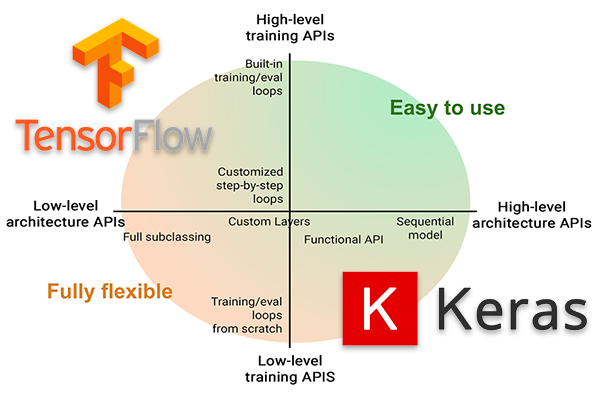
\includegraphics[width=0.8\linewidth]{images/keras.png}
    \caption{TensorFlow vs Keras Architecture}
    \label{fig:keras}    
\end{figure*}


\section{Backend Technologies}

\subsection{Node JS}

NodeJS enables the execution of JavaScript code outside the limitations of a web browser. It is cross-platform JavaScript runtime that allows for the creation of
fast and scalable network applications. Because of its architecture, that is asynchronous and event-driven, it handles concurrent operations efficiently, preventing the halt of
other processes. It suits real-time applications that are data-heavy and operate on a distributed network of devices. \cite{nodejs}

\subsubsection*{Advantages of Node.js}
NodeJS is designed as an asynchronous, event-driven JavaScript runtime ideal for crafting scalable network applications. Its efficiency and lightweight nature make it an excellent option for data-heavy, real-time applications.\cite{tilkov}
A significant benefit of NodeJS is its use of a single-threaded event loop, enabling it to manage multiple operations concurrently without hindering the execution of additional tasks.

A key feature of NodeJS is its extensive library ecosystem. The Node Package Manager (NPM) hosts over a million packages, making it the world's largest collection of open-source libraries.\cite{npm} 
This abundance of resources significantly streamlines the development process, allowing developers to leverage existing modules and focus on innovation.

NodeJS also benefits from its single programming language across both the server and client sides. This allows for the sharing of code and data between the server and the client, which is a great advantage, reducing the learning curve associated with NodeJS development. \cite{tilkov}
Furthermore, NodeJS's uniform programming language for both server and client sides simplifies code and data sharing across them, offering a streamlined learning process for development. In terms of performance, NodeJS excels due to its foundation on Chrome's V8 JavaScript engine, a high-performance engine that ensures speed and efficiency, especially in scenarios requiring real-time data processing. \cite{tilkov}

\subsubsection*{Disadvantages of Node.js}
NodeJS is not without its criticisms. Critics often point out the callback hell, a situation where the code becomes unreadable due to the excessive use of callbacks. Although it has been largely mitigated by the introduction of Promises and async/await syntax, it remains a valid criticism. \cite{cantelon2014node}

Table \ref{tab:node-js-advantages-disadvantages} is summarizing the advantages and disadvantages of Node.js\cite{tilkov}:

\begin{table}[H]
    \centering
    \begin{tabularx}{\textwidth}{|X|X|}
        \hline
        \textbf{Advantages of Node.js}                                                                                                               & \textbf{Disadvantages of Node.js}                                                                                                                              \\
        \hline
        Non-blocking and event-driven: Allows for scalabilityand concurrency, making it ideal for real-time applications.                    & Single-threaded: it is single-threaded, and can lead to blocking if not handled correctly, impacting CPU-bound tasks.                                   \\
        \hline
        JavaScript as a single language: It can be used for the server-side and client-side development, reducing context switching. & Callback hell: the code could be hard to read and maintain as there are nested callbacks (Promises and async/await can minimize this problem).                      \\
        \hline
        Large and active community: The Node Package Manager makes thousands of open-source libraries and modules available.                 & Limited support for multi-core processors: Node.js does not fully utilize multi-core CPUs out of the box.                                                      \\
        \hline
        Speed: it is known by its high-performance.                                               & Not weel suited for CPU-intensive tasks: The event-driven and single-threaded characteristics.           \\
        \hline
        Lightweight and fast startup: Node.js applications typically have lower memory consumption and quicker startup times.                        & Maturity and stability: Some developers argue that Node.js, compared to more established platforms, may have less maturity and stability in certain use cases. \\
        \hline
    \end{tabularx}
    \label{tab:node-js-advantages-disadvantages}
    \caption{Advantages and Disadvantages of Node.js}
\end{table}



\subsection{PM2}
PM2, or Process Manager 2, is a process manager for Node.js applications.
With a rich feature set, including monitoring, load balancing, and error handling, its primary function is to keep applications alive forever, restart them without downtime, and simplify common system administration tasks.
The standout feature of PM2 is its ability to keep processes running in the background indefinitely. This is particular important for web applications that requires constant availability. PM2 automatically resurrects crashed applications, ensuring that system glitches do not result in prolonged downtime.\cite{pm2}
This automatic restart capability is a safeguard against potentially costly application crashes that could otherwise lead to a poor user experience or even lost revenue. \cite{pm2}
PM2 also provides a built-in load balancer that can distribute incoming requests across multiple instances of the application. This improves performance and scalability, allowing the application to handle more requests, evenly distributing traffic across the instances, which can be particularly beneficial when running on multi-core systems. \cite{pm2LoadBalancing}
However, PM2 is not one-size-fits-all solution. It is designed for NodeJS applications, and is not suitable for applications written in other languages. It is also not suitable for applications that require a high degree of customization. \cite{pm2}
Despite the considerations, PM2's benefits have outweighed its limitations, and it was chosen as the technology for the project. It provides many features, including monitoring, load balancing, and error handling.
Its installation and setup process is straightforward, requiring minimal configuration. 
All these features make PM2 an ideal choice for the project, as it provides the necessary tools to manage and monitor the NodeJS application in a production environment.\cite{tilkov}

\subsection{Docker}

Docker is a tool that enables the creation, deployment, and running of applications in containers. 
Comparing with virtual machines (VMs), containers are lightweight, portable, and efficient, making them an ideal solution for deploying applications across different environments, 
having the application and its dependencies packaged into a single container. The containerization process encapsulates the application's code, the libraries, and the dependencies 
into a single object, ensuring that the application runs reliably and consistently across different environments. \cite{merkel2014docker}
Due to its simplicity and portability, Docker has become the de facto standard for containerization. Its lightweight nature compared to traditional virtual machines makes it ideal for cloud computing. 
The memory footprint is significantly reduced, and the performance is improved, making it an ideal solution for deploying applications in the cloud. \cite{merkel2014docker}

\begin{figure}[ht]
    \centering
    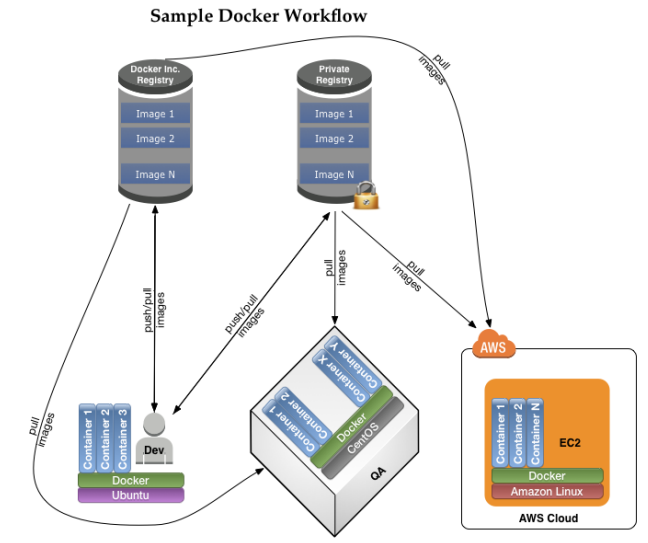
\includegraphics[width=0.8\linewidth]{images/docker.png}
    \caption{Development workflow with Docker}
    \label{fig:docker}
\end{figure}

However, Docker's container model is not without challenges. In the context of this project, the average size of a single Docker image exceeding 400MB presents a concern regarding bandwidth utilization. Continuous build and deployment processes involving large container images can consume substantial network resources, leading to potential cost overruns. \cite{merkel2014docker}
Another challenge is the security of Docker containers. Docker containers share the same kernel, which means that a vulnerability in the kernel can affect all containers. \cite{dockerhub}
While Docker's layering and image caching mechanisms can mitigate some of the network overhead, it is still a concern.
In conclusion, Docker is a powerful tool that offers numerous benefits for application deployment, from development to production. However, it is not without its challenges. The large size of Docker images can lead to bandwidth utilization issues, and the shared kernel model can lead to security concerns. Considering the scope of the project, time constraints and budget, Docker wasn't chosen as the technology for the project as the cost would be too high.


\subsection{NGINX}
NGINX works as a reverse proxy server, load balancer, and HTTP cache. It is a web server able to handle high volumes of concurrent connections,
which makes it an ideal solution for applications that require high availability and scalability. It is also lightweight and efficient
and highly configurable, allowing for the customization of its behaviour to suit the needs of the application.

It was created in 2004, with the goal of solving the C10K problem, refering to the challenge of handling 10,000 concurrent connections. \cite{nginx}
Due to its vast capabilities, and the ability to handle high volumes of concurrent connections, NGINX has become one of the most widely used web servers in the world,
often used as a load balancer and as a reverse proxy in addition to its role as a web server.

Table \ref{tab:ngnix} is showing some of the features of NGINX\cite{nginx}:

\begin{table}[H]
    \centering
    \begin{tabularx}{\textwidth}{|l|X|}
        \hline
        \textbf{Aspect}        & \textbf{Description}                                                                                                                      \\
        \hline
        Type                   & Web server software                                                                                                                       \\
        \hline
        Primary Use            & Serving web content, load balancing, reverse proxy, and more                                                                              \\
        \hline
        Performance            & Highly efficient in handling high concurrency with low memory footprint                                                                   \\
        \hline
        Architecture           & Event-driven, asynchronous, and non-blocking which contributes to its ability to handle a large number of simultaneous connections easily \\
        \hline
        Scalability            & Scalable to support growth in traffic and applications                                                                                    \\
        \hline
        Security Features      & Offers robust security features including rate limiting, client request filtering, and SSL/TLS termination                                \\
        \hline
        Flexibility            & Highly configurable for many type of servers                                                                       \\
        \hline
        Open Source/Commercial & Available in both open-source and commercial versions (NGINX Plus)                                                                        \\
        \hline
    \end{tabularx}
    \label{tab:ngnix}
    \caption{NGINX Features}
\end{table}

Due to its vast capabilities NGNIX was chosen for our project as reverse proxy and load balancer. It is an ideal solution for applications that require high availability and scalability with a 
high number of concurrent connections. It is also highly configurable, allowing for the customization of its behaviour to suit the needs of the application.

\subsection{MySQL}
MySQL uses structured query language (SQL) for database access, providing high performance and reliability. It interacts with the database using SQL, which
is a standard language for accessing and managing databases. 


Table \ref{tab:mysql} is showing some of the features of MySQL\cite{mysql}:

\begin{table}[H]
    \centering
    \begin{tabularx}{\textwidth}{|l|X|}
        \hline
        \textbf{Aspect}          & \textbf{Description}                                                                                                   \\
        \hline
        Data Handling            & Efficiently manages large datasets, crucial for training machine learning models                                       \\
        \hline
        Query Performance        & Fast query execution, beneficial for data retrieval and preprocessing in machine learning workflows                    \\
        \hline
        Scalability              & Easily scales with data volume and complexity, supporting the growing needs of machine learning applications           \\
        \hline
        ACID Compliance          & Ensures data integrity and consistency, vital for the accuracy of machine learning outputs                             \\
        \hline
        Advanced Analytics       & Supports SQL extensions for advanced analytics, facilitating machine learning data processing tasks                    \\
        \hline
        Data Storage Options     & Offers various storage engines, allowing optimization based on the specific needs of machine learning models           \\
        \hline
        Integration Capabilities & Easily integrates with popular machine learning frameworks and languages, streamlining the development process         \\
        \hline
    \end{tabularx}
    \label{tab:mysql}
    \caption{MySQL}
\end{table}

In the context of this project, the dataset was originally in a JSON format in FireStore which were found to be of a high complexity while performing compound querying. To facilitate querying and the 
difficulties of FireStore, MySQL was chosen to be the database for the project, where all the data for analysis is sourced directly from it, having a replica of the database
from the Legacy System. \\
By regularizing the data in MySQL, a more standardized and organized dataset was achieved. This standardization significantly simplified the data preprocessing steps in the machine learning workflow.


\subsection{Express JS}
Express.js, often simply called Express, is a streamlined and adaptable framework for Node.js designed to enhance web and mobile application development. It comes equipped 
with tools and features to suit every developers needs, while creating sophisticated applications.
It is often used to build server-side applications and APIs, due to its simplicity, performance, and scalability.In this project, Express.js was chosen for several strategic reasons, which are outlined below.\cite{express}

\begin{table}[H]
    \centering
    \begin{tabularx}{\textwidth}{|l|X|}
        \hline
        \textbf{Feature}     & \textbf{Advantage for Our Project}                                                                                                                              \\
        \hline
        Minimalist Framework & Express.js provides essential web application features without dictating any specific architecture, allowing for flexibility and customization in our project.  \\
        \hline
        Middleware Support   & The use of middleware modules enables us to extend the functionality of our application easily and efficiently.                                                 \\
        \hline
        Routing System       & Its powerful routing system helps manage requests and responses effectively, a crucial aspect for our project's RESTful API design.                             \\
        \hline
        High Performance     & Known for its high performance, Express.js enhances the responsiveness and speed of our web application.                                                        \\
        \hline
        Community Support    & As it is a very popular framework, it has strong community support, with many resources available.\\
        \hline
        Easy Integration     & Express.js seamlessly integrates with other technologies and databases, which is vital for the diverse tech stack of our project.                               \\
        \hline
        Simplicity           & Its simplicity and ease of use accelerate development and reduce the learning curve for new team members.                                                       \\
        \hline
    \end{tabularx}
    \label{tab:expressJS}
    \caption{Express.js Features}
\end{table}

It was chosen as a back end web application for this project due to its simplicity, performance, and scalability. Being widely used for building APIs and server-side applications, it offers a great
advantage.


\section{Testing Technologies}

\subsection{MochaJS}

Mocha is a JavaScript testing framework that runs in the browser and on Node.js. It executes sequentially, allowing for flexible and accurate testing of code. It accurately 
associates test results with the code that was tested, making it easier to identify and resolve issues. 
This testing framework has numerous features, offering functionalities such as asynchronous test execution, test coverage reports, and the ability to run tests in parallel.
Mocha is highly extensible, allowing for the integration of additional libraries and plugins to enhance the testing process. It supports a
variety of assertion libraries, giving the developer the option to choose the one that best suits. 

Mocha is widely used in the industry and is widely supported by the developer community. \cite{mocha}

\begin{table}[H]
    \centering
    \begin{tabularx}{\textwidth}{|l|X|}
        \hline
        \textbf{Feature}     & \textbf{Advantage for Our Project}                                                                                                                                  \\
        \hline
        Asynchronous Testing & Mocha's support for asynchronous testing was invaluable for testing our application's asynchronous operations, ensuring accurate and efficient tests.                   \\
        \hline
        Flexible Reporting   & Its variety of reporting options allowed us to choose the best format for our testing outcomes, enhancing readability and understanding of test results.               \\
        \hline
        Rich Assertion Library & Integration with various assertion libraries gave us the flexibility to write test cases in a style that best suited our project's needs.                          \\
        \hline
        Before/After Hooks  & Mocha's before and after hooks simplified the setup and teardown processes for our test suites, making our tests cleaner and more reliable.                           \\
        \hline
        Wide Adoption       & Mocha's popularity and wide adoption provided us with extensive resources for learning and troubleshooting, contributing to a smoother testing process.                 \\
        \hline
        Easy Integration    & Its seamless integration with other tools and libraries in our project's ecosystem allowed for a more streamlined development and testing workflow.                    \\
        \hline
        Customizable and Extensible & Mocha's customizable and extensible nature enabled us to adapt the testing to meet our project's specific requirements, enhancing test efficiency and effectiveness. \\
        \hline
    \end{tabularx}
    \label{tab:mochaTesting}
    \caption{Mocha Features and Advantages}
\end{table}

Mocha was selected for the testing of our project due to its flexibility, ease of use, and vast number of features suited for both synchronous and asynchronous tests. 

Throughout the development cycle, Mocha facilitated a robust testing environment that improved code quality and reliability. By utilizing Mocha's features, we were able to 
implement testing that covered a range of functions, allowing to identify and resolve issues early in the development process. 
Also, the ability to use different assertion libraries enabled our team to write test cases in a style that best suited our project's needs.

Mocha has proven to be an invaluable asset to our project, significantly enhancing our testing practices. Its adaptability, and vast documentation available online contributed 
to a higher quality final product.


\section{Difficulties}

The project faced a few challenges during the development process. The main one that affectted mostly the front end development was the deployment constraints on the virtual machine.
The deployment phase was challenging due to the resource intensive of our initial technology stack with Angular, Chart.js, Express JS, and Node JS. The virtual machine was not able
to handle the load of the application, which resulted in slow performance and frequent crashes. This led to the decision to switch to a more lightweight technology stack, 
which included EJS, Espress, CORS and AXIOS. This change improved the performance of the application and resolved the deployment issues.

\subsection{Embedded JavaScript (EJS)}
EJS is a straightforward templating language that enables the creation of HTML markup using pure JavaScript. It provides a rendering mechanism for dynamically generating HTML content.\cite{ejs}
Its compatibility with Express.js allows for it to render data from the server-side to the client-side, making it an ideal choice for web application development. 
EJS also allows to reuse of code snippets, increasing the efficiency of web application development. 
It also allows for the implementation of conditional logic, enabling the rendering of different content based on specific conditions. EJS supports looping constructs, facilitating the iteration over data collections 
and the generation of repetitive HTML elements. It provides error handling capabilities, ensuring that errors are caught and managed effectively during the rendering process. EJS is highly extensible,
allowing for the integration of additional features and functionalities to enhance the rendering process. \cite{ejs}

\begin{table}[H]
    \centering
    \begin{tabularx}{\textwidth}{|l|X|}
        \hline
        \textbf{Feature}     & \textbf{Description}                                                                                                                              \\
        \hline
        Simple Syntax       & EJS uses a simple syntax that allows for the embedding of JavaScript code within HTML markup.                                                      \\
        \hline
        Dynamic Content     & EJS enables the dynamic generation of HTML content.                      \\
        \hline
        Code Reusability    & EJS supports the reuse of code snippets, enhancing the efficiency of web application development.                                                    \\
        \hline
        Conditional Logic   & EJS allows for the implementation of conditional logic, enabling the rendering of different content based on specific conditions.                      \\
        \hline
        Looping Constructs  & EJS supports looping constructs, facilitating the iteration over data collections and the generation of repetitive HTML elements.                      \\
        \hline
        Error Handling      & EJS provides error handling capabilities, ensuring that errors are caught and managed effectively during the rendering process.                         \\
        \hline
        Extensibility       & EJS is highly extensible, allowing for the integration of additional features and functionalities to enhance the rendering process.                      \\
        \hline
    \end{tabularx}
    \label{tab:ejs}
    \caption{EJS Features}
\end{table}

\section{Security}
Security is a critical aspect of any application, especially when dealing with sensitive data. In the context of this project, security measures were implemented 
to protect the application from potential threats and vulnerabilities. Among the various security measures available, JSON Web Tokens (JWT) was chosen for securely
transmitting information between parties as JSON objects. 

\subsection{JSON Web Tokens - JWT}

JWTs play a crucial role in authentication and authorization processes. A key advantage of JWTs lies in their capability to securely and efficiently transmit information
between parties as JSON objects. 
The structure of a JWT comprises three fundamental components: a header, a payload, and a signature. The header provides details about the token type and the algorithm used to sign it.
The payload contains claims, which are statements about an entity along with additional data. Lastly, the signature is utilized for verifying the authencity of the JWT sender
and ensuring the integrity of the message throughout its transmission. \cite{jwt}.

\textbf{Utilizing the Token}: Once the client possesses the token, it can be included in the header of the HTTP request to the server, which can then verify 
the token and grant access to the requested resource if the token is valid.

\textbf{Assessing Token Validity}: Receiving a token does not guarantee its validity. The token is verified by the server to make sure that it has not been tampered with
and that it is still valid. This process involves checking for token signature and the payload claims. 

This is done by checking the signature of the token and verifying the claims in the payload.

\textbf{Decision on Access}: If the token is valid, the server can grant access to the requested resource. If the token is invalid, the server can deny access.

\textbf{Token Expiration}: Expiration time can be set for JWTs, after which they are no longer valid. This helps to prevent the misuse of tokens and enhances security.



